
\section{Misleading Generalized Itemsets}\label{mgi_intro}
%
%In the last few years the new Information and Communication Technologies (ICT) have supported cities in becoming smart.
%Hence, the capability of smart cities to generate and collect data of public interest (e.g., information about social events, public service usage, traffic law infractions) has increased at an unprecedented rate, 
%to such an extent that data rapidly scales towards ``Big Data''. 
%
%Big Data analyses are challenging tasks because the computational cost of data mining processes is often very high and, in some cases, prohibitive
%on a non-distributed system.  Hence, relevant research efforts have been devoted to large-scale data mining based on the MapReduce paradigm~\cite{Dean2008}.
%Data mining encompasses a large variety of techniques, such as cluster analysis, frequent pattern extraction, and classification~\cite{KumarBook}. 
%For example, some remarkable attempts to address itemset and association rule mining from Big Data have recently been made (e.g.,~\cite{pfpgrowth,bigfim,ISPA13,PMINE13}). 
In this second part of the Chapter, as already mentioned, we will extend the discussed distributed network data mining framework to focus on an established pattern mining technique called generalized itemset extraction~\cite{Srikant1995}. The obtained architecture framework has been named \SeTAB\ (\SeTA )
This technique has already been applied to data coming from different application domains (e.g., market basket analysis~\cite{Srikant1995}, network traffic data analysis~\cite{IS2010}, genetic data mining~\cite{BaralisCCCG13}). 
Generalized itemset mining entails discovering correlations among data at different abstraction levels. By exploiting a taxonomy (i.e., a set of is-a hierarchies) built over the analyzed data, 
frequent generalized itemsets, which represent recurrent co-occurrences among data items at different granularity levels, are extracted. 
These patterns are worth considering by domain experts to transform huge amounts of raw data into useful and actionable knowledge. 
However, a subset of peculiar high-level patterns should be analyzed separately during manual result inspection.  
More specifically, each generalized itemset has a correlation type which indicates the strength of the correlation between the corresponding items. 
Misleading Generalized Itemsets (MGIs)~\cite{MGI} are generalized itemsets
whose correlations type is in contrast to those of most of their low-level descendant itemsets.
These high-level patterns are worth considering for in-depth analysis because they are likely to represent misleading and thus potentially interesting situations. 
In~\cite{MGI} MGI extraction is performed in main memory on top of frequent level-sharing itemsets. 
Unfortunately, when coping with Big Datasets, a large number of itemsets is often generated at step (i) thus MGI extraction becomes a challenging task. 
However, to the best of our knowledge, no attempt to mine MGIs on a distributed architecture has been made yet. 

The remainder part of this Chapter presents \SeTAB\ (\SeTA ), an instance of the more general framework \Nemico\ designed to efficiently mine MGIs on a distributed computing model. 
%To efficiently cope with Big Data collections, the system implementation is distributed and most operations are mapped to the MapReduce programming paradigm~\cite{Dean2008}. 
%As a reference case study, the proposed approach has been applied to a real application context: the analysis of the traffic law infractions committed by 
%the citizens of Turin, an important business and cultural centre in northern Italy. 
%Real infraction data is provided as open data by the Turin administration.
%The goal of the analysis is to improve the efficiency of public services, 
%the transparency of public administrations, and the awareness of the degree of civilization of urban people.
The experimental results show the effectiveness and efficiency of the \SeTAB\ architecture as well as they demonstrate its applicability to the analyzed use-cases. 



%*********************************************************
\section{Related work}
\label{relwork}
%*********************************************************

In the last years, a relevant research effort has been devoted to large-scale itemset mining based on the MapReduce paradigm~\cite{Dean2008}. 
The goal is to propose itemset extraction algorithms that distribute data and computation across a distributed architecture to scale the mining process towards Big Data~\cite{pfpgrowth,bigfim,ISPA13}.
%A parallel version of an established itemset mining algorithm, i.e., FP-Growth, has first been proposed in~\cite{pfpgrowth}. 
%The algorithm, named PFP, consists of two separate MapReduce jobs 
%and it achieves an almost linear speedup.
%It converts transactions of the original database into some new databases of group-dependent transactions so that local FP-trees built
%from different group-dependent transactions can be separately processed during the recursive conditional FP-tree constructing process. 
%For each group PFP extracts top-k frequent itemsets (i.e., a subset of frequent itemsets).
%More recently, two new methods, namely Dist-Eclat and BigFIM, for mining all frequent itemsets from large datasets 
%have been presented in~\cite{bigfim}. 
%Specifically, Dist-Eclat focuses on improving algorithm speed, while BigFIM is optimized to run on huge datasets.
%In parallel, a cloud-based service for association rule mining from network traffic data has been presented in~\cite{ISPA13}.
Unlike aforementioned papers, this works investigates the applicability of a generalized pattern mining technique on the MapReduce platform. 

\textbf{TO DO: still to be rephrased}

The frequent generalized frequent itemset and association rule mining problems~\cite{Srikant1995} have largely been studied by the data mining community.
The firstly proposed approach~\cite{Srikant1995} generates itemsets by considering for each item all its ancestors in the taxonomy. 
To avoid generating all the possible itemsets, the authors in~\cite{Sriphaew2002,BaralisCCG12} proposed to push (analyst-provided) constraints into the mining process.
In parallel, many algorithm optimizations and variations have been proposed~\cite{Han1999,KunkleZC08,ChangeTKDE}. 
For example, the approach presented in~\cite{Han1999} proposes an optimization strategy based on a top-down hierarchy traversal, while 
in~\cite{KunkleZC08} the authors propose to mine closed and maximal generalized itemsets. 
More recently, a new type of generalized pattern, called Misleading Generalized Itemset (MGI), has been proposed~\cite{MGI}. 
MGIs are high-level (generalized) itemsets for which a relevant subset of frequent descendants have a correlation type in contrast to their common ancestor. 
MGIs are worth considering separately from traditional itemsets if their low-level contrasting correlations cover almost the same portion of data as the high-level itemset, 
because the information provided by traditional high-level patterns becomes misleading. 
Unlike~\cite{MGI}, this paper investigates how to perform MGI mining on the MapReduce platform. 
Furthermore, it evaluates the MGIs extracted big data acquired in smart city and networking environments.


%**********************************************************
\section{Preliminary concepts and problem statement}
\label{probstat}
%**********************************************************

A relational dataset $\cal{D}$ consists of a set of records, where each record is a set of items~\cite{KumarBook}. Each item is a pair ($attribute$,~$value$).
A taxonomy $\Gamma$ built over the source dataset $\cal{D}$  aggregates the data items into higher-level concepts (i.e., the generalized items). 
Table~\ref{tab:example2} and Table~\ref{fig:tax} report two representative examples of relational dataset and taxonomy, respectively, which hereafter will be used as running examples. 
%
%\begin{table*}%
%\parbox{0.42\textwidth}{
%\caption{Example dataset $\cal{D}$ after discretization.}
%\begin{scriptsize}
%\begin{center}
%\begin{tabular}{|c||c|c|}
%\hline {\bf Rid} & {\bf Infraction name} & {\bf time stamp} \\
%\hline
%\hline 1 & One-way infraction & [8 a.m.,9 a.m.] \\
%\hline 2 & One-way infraction & [8 a.m.,9 a.m.] \\
%\hline 3 & Speeding & [8 a.m.,9 a.m.] \\
%\hline 4 & Driving without license & [9 a.m.,10 a.m.] \\
%\hline 5 & Driving without license & [9 a.m.,10 a.m.] \\
%\hline 6 & Unfastened seat belt & [4 p.m.,5 p.m.] \\
%\hline 7 & One-way infraction & [8 a.m.,9 a.m.] \\
%\hline
%\end{tabular}
%\end{center}
%\end{scriptsize}
%\label{tab:example2}
%\vspace{1cm}
%}
%\qquad
%\begin{minipage}[c]{0.37\textwidth}%
%\centering
%\caption{Example taxonomy built over items in $\cal{D}$}
%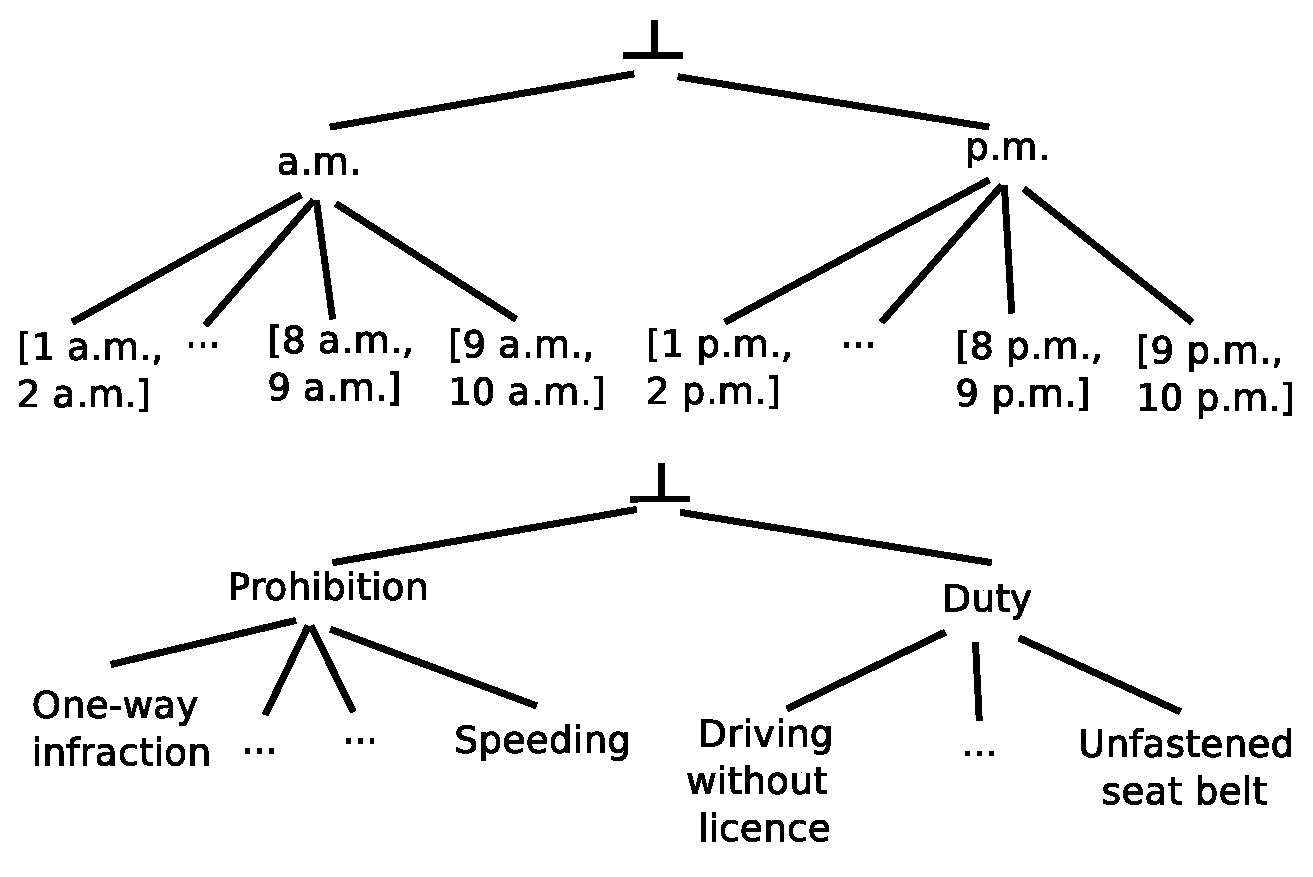
\includegraphics[width=\textwidth]{chapters/mgi/gerarchia/GerarchiaISPATre.eps}
%\label{fig:tax}
%\end{minipage}
%\end{table*}

\begin{figure}
\centering
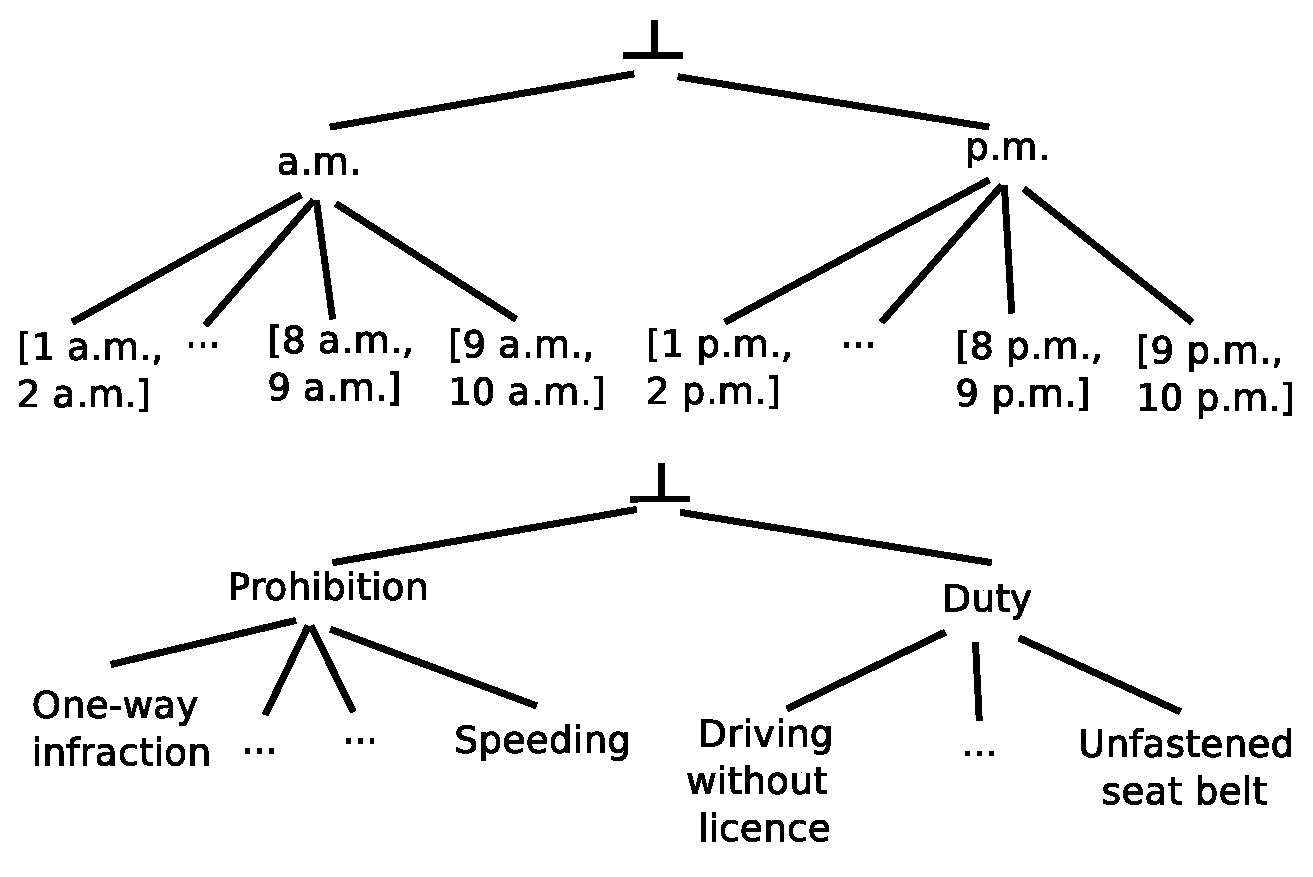
\includegraphics[width=0.60\textwidth]{chapters/mgi/gerarchia/GerarchiaISPATre.eps}
\caption{Example taxonomy built over items in $\cal{D}$}
\label{fig:tax_net}
\end{figure} 

\begin{table*}[th!]
%\scriptsize
\caption{\MGI{}s mined from $\cal{D}$. min\_sup = 10\%, max\_neg\_cor= 0.70, min\_pos\_cor= 0.80, and max\_NOD = 80\%.} \label{tab:exampleMGI}
\centering
\hspace{-1.5cm}
\begin{tabular}{|c||c|c|}
\hline {\bf Rid} & {\bf Infraction name} & {\bf time stamp} \\
\hline
\hline 1 & One-way infraction & [8 a.m.,9 a.m.] \\
\hline 2 & One-way infraction & [8 a.m.,9 a.m.] \\
\hline 3 & Speeding & [8 a.m.,9 a.m.] \\
\hline 4 & Driving without license & [9 a.m.,10 a.m.] \\
\hline 5 & Driving without license & [9 a.m.,10 a.m.] \\
\hline 6 & Unfastened seat belt & [4 p.m.,5 p.m.] \\
\hline 7 & One-way infraction & [8 a.m.,9 a.m.] \\
\hline
\end{tabular}
\end{table*}

%
%
%\begin{table}%
%%\centering
%\parbox{0.45\textwidth}{
%\begin{scriptsize}
%\begin{tabular}{|c||c|c|}
%\hline {\bf Rid} & {\bf Port Number} & {\bf RTT} \\
%\hline
%\hline 1 &  Port 80 & [0 - 50 ms] \\
%\hline 2 &  Port 80 & [0 - 50 ms] \\
%\hline 3 &  Port 443 &[0 - 50 ms]\\
%\hline 4 & Port 2009 & [50 - 100 ms] \\
%\hline 5 & Port 2009 & [50 - 100 ms] \\
%\hline 6 & Port 53066 &[150 - 200 ms] \\
%\hline 7 & Port 80 & [0 - 50 ms]\\
%\hline
%\end{tabular}
%\end{scriptsize}
%\vspace{1cm}
%\caption{Example dataset $\cal{D}$ after discretization.}
%\label{tab:example2_net}
%}
%\qquad
%\hspace{-0.6cm}
%\begin{minipage}[c]{0.53\textwidth}%
%%\centering
%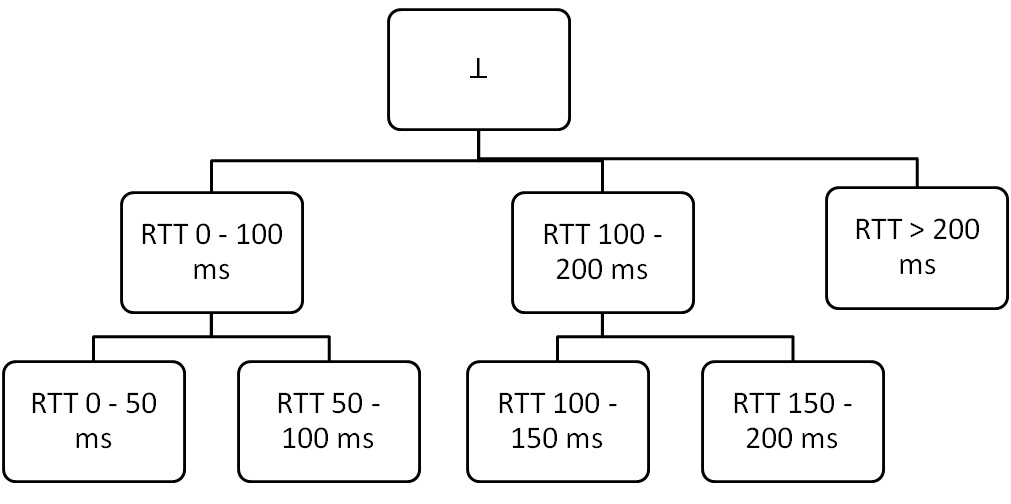
\includegraphics[width=\textwidth]{chapters/mgi/tass_collage.jpg}
%\caption{Example taxonomy built over items in $\cal{D}$}
%\label{fig:tax_net}
%\end{minipage}
%\end{table}


\begin{table*}[th!]
\scriptsize
\caption{\MGI{}s mined from $\cal{D}$. min\_sup = 10\%, max\_neg\_cor= 0.70, min\_pos\_cor= 0.80, and max\_NOD = 80\%.} \label{tab:exampleMGI}
\centering
\hspace{-1.5cm}
\begin{tabular}{|c|c|c|}
\hline 
 {\bf Frequent}       		& {\bf Frequent}                   & {\bf Not }    \\
 {\bf itemset (level$\geq$2)}    		& {\bf descendants}                 & {\bf overlapping} \\
 {\bf [correlation type (Kulc value)]}   	& {\bf [correlation type (Kulc value)]} &  {\bf degree (\%)}         \\
\hline
$\{$ (Time, a.m.), (Infraction name, Prohibition)$\}$    &   $\{$(Time, [8 a.m.,9 a.m.]), (Infraction name, One-way infraction)$\}$ & 75   \\
     \textit{[positive (5/6=0.83)]}       &    \textit{[positive (7/8=0.88)]}         &  \\
                                 &  $\{$(Time, [8 a.m.,9 a.m.]), (Infraction name, Speeding)$\}$    &  \\
                                 &    \textit{[[negative (5/8=0.63)]}              &  \\
\hline
 $\{$(Time, a.m.), (Infraction name, Duty)$\}$  &  $\{$(Time, [9 a.m., 10 a.m.]), (Infraction name, Driving without license)$\}$  & 0  \\
           \textit{[negative (1/2=0.50)]}                  & \textit{[positive (1)]} &  \\        
\hline
 $\{$(Time, p.m.), (Infraction name, Duty)$\}$  &  $\{$(Time, [4 p.m.,5 p.m.]), (Infraction name, Unfastened seat belt)$\}$  & 0   \\
           \textit{[negative (2/3=0.66)]}                  &  \textit{[positive (1)]} &  \\
\hline
\end{tabular}
\end{table*}



A $k$-itemset is a set of $k$ (generalized) items. 
For example, \{(\textit{Time},\textit{a.m.}), (\textit{Infraction name},\textit{One-way infraction})\} is a $2$-itemset, 
which indicates that the two items co-occur (possibly at different abstraction levels) in the source data.  
Items/itemsets are characterized by many notable properties~\cite{Srikant1995}, such as support, coverage, descent and level of abstraction according to an input taxonomy $\Gamma$. 
For their definitions please refer to~\cite{Srikant1995,Han1999,MGI}. 
Similar to~\cite{Han1999,Flipping}, we target the correlations among items at same abstraction level, i.e. the itemsets that exclusively contain items with the same level. Such patterns are denoted by \textit{level-sharing itemsets}~\cite{Han1999}. 

The itemset correlation measures the strength of the correlation between its items. Similar to~\cite{Flipping}, in this paper
we evaluate the correlation of a $k$-itemset $I$ by means of the Kulczynsky (Kulc) correlation measure~\cite{Wu2010Interestingness}
Kulc values range from 0 to 1. By properly setting maximum negative and minimum positive
Kulc thresholds, hereafter denoted by \textit{max\_neg\_cor} and \textit{min\_pos\_cor}, the itemsets may be classified as negatively correlated, uncorrelated, or positively correlated itemsets according to their correlation value.  

Let $\mathcal{LSI}$ be the set of all frequent level-sharing itemsets in $\mathcal{D}$ according to a minimum support threshold min\_sup. 
Given a frequent level-sharing itemset $X \in \mathcal{LGI}$ of level $l\geq2$, let 
Desc$^*$[$X$,$\Gamma$] be the subset of corresponding level-($l-1$) $X$'s descendants for which the correlation type is in contrast to those of $X$. 
A \MGI\ (MGI) is a pattern in the form $X \triangleright \mathcal{E}$, where $X \in \mathcal{LSGI}$ and $\mathcal{E}$=Desc$^*$[$X$,$\Gamma$]~\cite{MGI}. 

For example, by enforcing min\_sup=10\%, max\_neg\_cor=0.70, 
and min\_pos\_cor=0.80, MGI
\{(Time,a.m.), (Infraction name,Prohibition)\}~$\triangleright$~\{(Time, [8 a.m.,9 a.m.]), (Infraction name,Speeding)\} is 
mined from the dataset in Table~\ref{tab:example2}, 
because \{(Time,a.m.), (Infraction name,Prohibition)\} has a positive correlation (0.83), 
whereas its descendant itemset \{(Time,[8 a.m., 9 a.m.]), (Infraction name,Speeding)\} is negatively correlated (0.63).

To measure the degree of interest of a MGI $X \triangleright \mathcal{E}$ with respect to its corresponding traditional itemset version ($X$), 
the Not Overlapping Degree (NOD) measure has been defined in~\cite{MGI}. 
The NOD of an MGI $X \triangleright \mathcal{E}$ is defined as 
$\frac{\mbox{sup}(X,\cal{D})-\mbox{cov}(\mathcal{E},\cal{D})}{\mbox{sup}(X,\cal{D})}$.
It expresses the relative difference between the support of the ancestor itemset $X$ and the coverage of its low-level contrasting correlations in $\mathcal{E}$.
The NOD values range from 0 to 1. The lower NOD value we achieve, the more significant the degree of overlapping between 
the contrasting low-level correlations in $\mathcal{E}$ and their common ancestor $X$ becomes. 

The mining task addressed by this paper entails discovering from $\cal{D}$ all the MGIs for which
the NOD value is less than or equal to a maximum threshold max\_NOD. The subset of \MGI s mined from Table~\ref{tab:example2} by setting the maximum NOD threshold to 80\% is reported in Table~\ref{tab:exampleMGI}.




%**********************************************************
\section{The \SeTAB\ architecture}
\label{setarch}
%**********************************************************

The \SeTAB\ architecture provides a cloud-based service for discovering hidden and actionable patterns among potentially Big datasets.
We focus our analysis on two specific case studies, i.e., the analysis of the traffic law infractions committed in a urban environment and the Internet traffic generated by an Italian ISP. 
To efficiently cope with Big Data, the system implementation is distributed and most operations are mapped to the MapReduce programming paradigm~\cite{Dean2008}.
The architecture has been designed as a chain of distributed jobs running on an Hadoop cluster, as described below. 


%**********************************************
\subsection{Data retrieval and preparation}
\label{acquisitionprep}
%**********************************************

Data about traffic law infractions was collected by traffic engineers. 
Reports about daily infractions are collected in local data repositories, which are then integrated into open Big Datasets. 
A traffic law infraction dataset $\mathcal{D}$ consists of a set of records $r$, each one representing a different infraction. 
Each record is a set of \textit{items}, where items are pairs (\textit{attribute},\textit{value}). \
\textit{Attribute} can be a specific characteristic of the traffic law infraction (e.g.,  infraction name, law article) 
or a property of the context in which the infraction was committed (location, date, time), 
while \textit{value} is the value assumed by the corresponding attribute. 
Hereafter, for the sake of simplicity, we focus our analysis on the following attribute subset: \textit{Infraction name}, \textit{Vehicle type}, \textit{Location}, \textit{Date}, and \textit{Time}. 
We discretized time stamps (e.g., 8.10 a.m.) into 1-hour time slots (e.g., from 8 a.m. to 9 a.m.) using ad-hoc mapping functions. 
The dataset reported in Table~\ref{tab:example2} is already the output of the discretization step.

About the network traffic datasets, it has been obtained collecting network measuremets.
To this aim, a passive probe is
located on the access link (vantage point) that connects an
edge network to the Internet. The passive probe sniffs all
incoming and outgoing packets flowing on the link, i.e.,
packets directed to a node inside the network and generated
by a node in the Internet, and vice versa. The probe runs
Tstat~\cite{Tstat},~\cite{Tstat2}, a passive monitoring tool allowing network
and transport layer measurement collection. Tstat rebuilds
each TCP connection by matching incoming and outgoing
segments. Thus, a flow-level analysis can be performed~\cite{Tstat2}.
A TCP flow is identified by snooping the signaling flags
(SYN, FIN, RST). The status of the TCP sender is rebuilt
by matching sequence numbers on data segments with the
corresponding acknowledgement (ACK) numbers.
To evaluate the \SeTAB\ tool in real-world application, we focus on a subset of measurements describing the traffic flow among the many provided by Tstat. The most meaningful features, selected with the
support of domain experts, are detailed in the following:
\begin{itemize}
\item the Round-Trip-Time (RTT) observed on a TCP flow,
i.e., the minimum time lag between the observation of a
TCP segment and the observation of the corresponding
ACK. RTT is strongly related to the distance between
the two nodes.
\item the number of hops (Hop) from the remote node to
the vantage point observed on packets belonging to the
TCP flow, as computed by reconstructing the IP Time-
To-Live
\item the flow reordering probability (P{reord}), which can
be useful to distinguish different paths
\item the flow duplicate probability (P{dup}), that can highlight
a destination served by multiple paths
\item the total number of packets (NumPkt), the total number
of data packets (DataPkt), and the total number
of bytes (DataBytes) sent from both the client and
the server, separately (the client is the host starting the
TCP flow)
\item the minimum (WinMin), maximum (WinMax), and
scale (WinScale) values of the TCP congestion window
for both the client and the server, separately
\item the TCP port of the server (Port)
\item the class of service (Class), as defined by Tstat, e.g.,
HTTP, video, VoIP, SMTP, etc.
\end{itemize}
Based on measurements listed above, an input data record is
defined by the following features: RTT, Hop, P{reord},
P{dup}, NumPkt, DataPkt, DataBytes, WinMax,
WinMin, WinScale, Port, Class. To obtain reliable
estimates on reordering and duplicate probabilities, only
TCP flows which last more than P = 10 packets are
considered. This choice allow focusing the analysis on longlived
flows, where the network path has a more relevant
impact, thus providing more valuable information.\\
Since frequent itemset mining requires a transactional dataset of
categorical values, data has to be discretized before the mining.
The discretization step converts continuously
valued measurements into categorical bins. Then, data
are converted from the tabular to the transactional format.
As already mentioned, attribute selection and data discretization are performed as distributed MapReduce jobs (specifcally, as a single map only job). Each
record is processed by the map function and, if the number
of packets is above the threshold (10 packets), the corresponding
discretized transaction is emitted as a result of the
mapping. This task entails an inherently parallel elaboration,
considering that can be applied independently to each record.



%**********************************************
\subsection{Taxonomy generation}
\label{taxmapping}
%**********************************************

To analyze data from a high-level viewpoint, the datasets are equipped with taxonomies.
A taxonomy is a set of is-a hierarchies built over data items in $\mathcal{D}$. 
An example taxonomy built over the dataset in Table~\ref{tab:example2} is depicted in Table~\ref{fig:tax}. 
Items whose value is an high-level aggregation belonging to the taxonomy (e.g., (\textit{Infraction name},\textit{Duty})) are called \textit{generalized items}. 
In Figure~\ref{fig:tax_net}, instead, is reported a sample taxonomy over the attribute RTT of the network traffic dataset.

Analyst-provided taxonomies could be generated either manually or semi-automatically by domain experts. 

To perform our analyzes of the traffic law dataset, we built 3-level hierarchies over the contextual attributes (Location, Time, Date). Specifically, geographical addresses 
are aggregated into the zip code, which in turn are aggregated into the corresponding district; 1-hour time slots are generalized as the corresponding 4- and 12-hour time slots, 
while dates are generalized as the corresponding month and year.
Furthermore, vehicles are generalized as the corresponding category (e.g., \textit{Car}, \textit{Dumper track}, \textit{Pickup track}), and
infraction names are aggregated into the corresponding high-level class given by the public administration of Turin.
A similar process has been applied to network traffic dataset. There were few cases where it was not possible: for instance, Protocols attributes habe been grouped in classes based on use case domains (similar to \cite{grimaudo2012hierarchical}).

In this work we consider as input balanced taxonomies (i.e., taxonomies whose hierarchies have all the same height). 
If experts do not provide balanced taxonomies, a re-balancing procedure similar to those adopted in~\cite{Flipping} is applied prior to level-sharing itemset mining. 


\begin{figure}
\centering
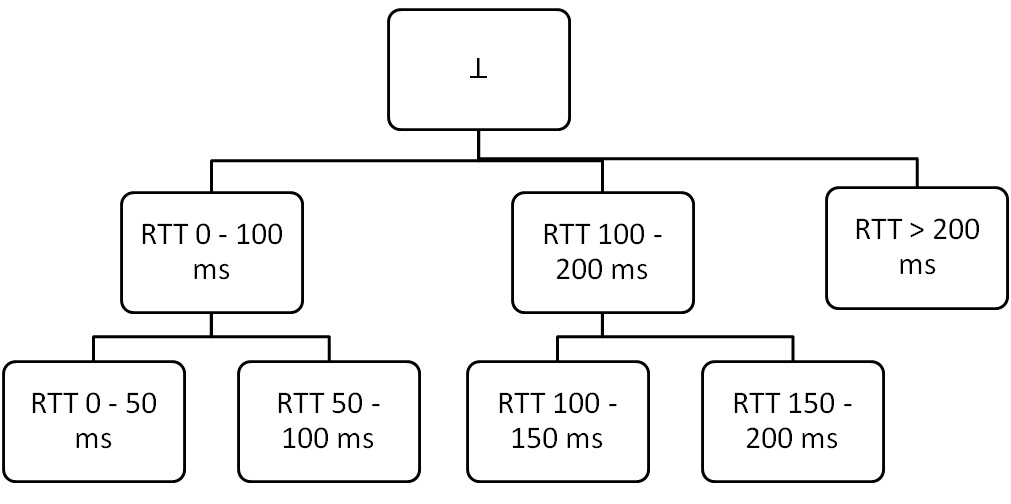
\includegraphics[width=0.60\textwidth]{chapters/mgi/tass_collage.jpg}
\caption{Example of taxonomie over RTT attribute}
\label{fig:tax_net}
\end{figure} 


%**********************************************
\subsection{Level-sharing itemset mining}
\label{levelsharing}
%**********************************************


Given a preprocessed infraction dataset and a minimum support threshold min\_sup, this job accomplishes the first MGI mining step, i.e., the extraction of all frequent level-sharing itemsets~\cite{Han1999}.  
This job performs the following tasks. 

\noindent \textbf{Dataset extension}. This task entails producing a new dataset version which integrates taxonomy information. 
To enable frequent level-sharing itemset mining from data containing items at different abstraction levels, it generates multiple copies of each record, one for each taxonomy level. 
While the original record contains only taxonomy leaves (i.e., the dataset items), each copy contains the corresponding combination of item generalizations at a different abstraction level.To avoid unnecessary I/O operations, the extended dataset version is not materialized on disk, but it is directly 
generated in the map function of the itemset extraction task and then immediately stored into a compact FP-tree structure~\cite{KumarBook}.

\noindent \textbf{Itemset extraction}. To efficiently mine frequent level-sharing itemsets~\cite{Han1999} from the extended dataset version, 
this task exploits a variation of the Hadoop-based itemset mining algorithm proposed in~\cite{ISPA13}. 


%**********************************************************
\subsection{MGI extraction}
\label{rulext}
%**********************************************************

This job performs MGI mining on top of the frequent level-sharing itemsets. 
Specifically, it accomplishes the task stated in Section~\ref{probstat}. 
This step consists of a MapReduce job, as described in the following.
The contribution of this job is new because, to the best of our knowledge, no cloud-based service currently supports MGI mining from Big Data.

To extract MGIs we combine each frequent level-sharing itemset $I$ with  
its corresponding set of descendant itemsets $\mbox{Desc}[I,\Gamma]$. 
More specifically, In the map function for each level-sharing itemset $I$, the following two pairs ($key$, $value$) are emitted:
(i) a pair ($key$, $value$), where $key$ is the direct ancestor of itemset $I$ and $value$ the itemset $I$ with its main properties (i.e., support and Kulc values) and
(ii) a pair ($key$, $value$), where $key$ is the itemset $I$ is the $value$: itemset $I$ with its main properties (i.e., support and Kulc values).
Two pairs are emitted because each itemset can be a descendant of an itemset and 
a parent of another one at the same time. The first pair allows us to associate $I$ with the ancestor key, whereas
the second pair is used to associate $I$ to itself if MGIs in the form $I \triangleright \mathcal{E}$ are extracted. 
The generated pairs allow us to map each itemset and its corresponding descendants to the same key. 
Hence, in the reduce function, each key is associated with a specific itemset $I$ and the corresponding set of values 
contains both the (ancestor) itemset $I$ and its respective descendants. By iterating on the set of values associated with key $I$, 
we generate candidate MGIs $I \triangleright \mathcal{E}$, where $\mathcal{E}$ is the set of $I$'s descendants in contrast to $I$ in terms of correlation type,
and we compute the corresponding NOD values. Finally, only the MGIs satisfying the max\_NOD threshold are stored into the HDFS file system.


%**********************************************************
\section{Experiments}
\label{exp}
%**********************************************************
We performed experiments on two real datasets acquired in different domains:

\noindent \textbf{AperTo dataset.}  This open dataset, available at http://aperto.comune.torino.it, collects information about approximately 2 millions of traffic law infractions committed in the city 
of Turin over the 3-year period 2011-2013. The dataset is characterized by five attributes (\textit{Infraction name}, \textit{Vehicle type}, \textit{Location}, \textit{Date}, and \textit{Time}). Its size is approximately 198 MB. 
Hierarchies over the infraction data items were defined according to the guidelines reported in Section~\ref{taxmapping}.

\noindent  \textbf{BigNetData dataset.} This relational network traffic dataset has been obtained by performing different
capture stages on a backbone link of a nation-wide ISP in Italy that offers us three different vantage points.
The dataset has size 192.56 GB and it consists of 413,012,989 records, i.e., one record for each bi-directional TCP flow).
A more detailed dataset description is given in~\cite{ISPA13}.

The MapReduce jobs of the \SeTAB\ workflow (see Section~\ref{setarch}) were
developed in Java using the new Hadoop Java APIs.
The experiments were performed on a cluster of 5 nodes running Cloudera's
Distribution of Apache Hadoop (CDH4.5). Each cluster node is a 2.67~GHz
six-core Intel(R) Xeon(R) X5650 machine with 32~Gbyte of main memory running
Ubuntu 12.04 server with the 3.5.0-23-generic kernel. All the reported
execution times are real times obtained from the Cloudera Manager web control panel.

In the experiments we addressed the following issues: 
(i) the analysis of the characteristics of the mining results achieved with different parameter settings ((Section~\ref{impactparam})), 
(ii) the validation of the usefulness of the results achieved for performing in-depth analysis (Section~\ref{validation}), 
and (iii)~the scalability of the MGI Miner algorithm with the number of nodes (Section~\ref{scalability}). 
We addressed Tasks (i) and (ii) mainly on AperTo dataset, because data fully complies with the context under analysis (i.e., infraction data analysis), whereas
Task (iii) was addressed on BiGNetData, because it is a larger dataset characterized by a fairly complex data distribution.

%**********************************************************
\subsection{Characteristics of the mining results}
\label{impactparam}
%**********************************************************

\begin{figure}[t]
\centering
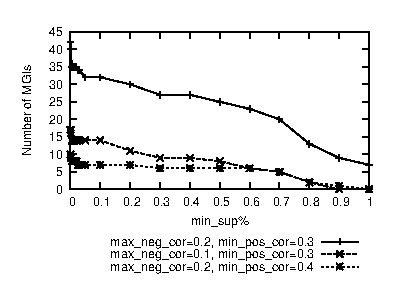
\includegraphics[width=0.32\textwidth]{chapters/mgi/grafici/EffectMinsup.eps}
\caption{Effect of the minimum support threshold. max\_NOD=60\%.}
\label{fig:minsup}
\end{figure}

\begin{figure}[t]
\centering
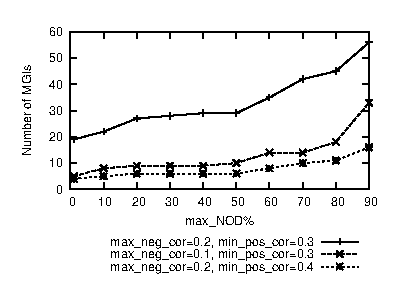
\includegraphics[width=0.32\textwidth]{chapters/mgi/grafici/EffectMaxNOD.eps}
\caption{Effect of the maximum NOD threshold. minsup=0.02\%.}
\label{fig:maxnod}
\end{figure}

We analyzed the impact of the main input parameters of the MGI Miner algorithm on the number of MGIs mined.
Figure~\ref{fig:minsup} summarizes the number of mined MGIs by varying the minimum support threshold (min\_sup) for different combinations of minimum positive and maximum negative correlation thresholds (max\_neg\_cor and  min\_pos\_cor, respectively), 
while Figure~\ref{fig:maxnod} shows the number of mined MGIs by varying the max\_NOD threshold for the same combinations of correlation threshold values.

The number of mined MGIs non-linearly increases by decreasing the minimum support threshold due to the combinatorial increase in the number of generated frequent itemsets~\cite{Agr94}. 
Since most itemsets have correlation between 0.1 and 0.3, the maximum number of MGIs is extracted if max\_neg\_cor and min\_pos\_cor fall in this value range, 
because the generalization process is most likely to flip the itemset correlation types. As expected, the smaller the gap between max\_neg\_cor and min\_pos\_cor, 
the more MGIs are extracted because correlation type changes occur, on average, more frequently. 
For all the tested configurations, the set of mined MGIs remains still manageable by domain experts for manual inspection even while setting relatively low support thresholds (e.g., 35 MGIs mined with max\_neg\_cor=0.2, min\_pos\_cor=0.3 and min\_sup=0.01\%). 

The number of mined MGIs non-linearly increases while increasing the maximum not overlapping degree threshold max\_NOD, because low-level itemsets are more likely to cover a significant portion of data already covered by the corresponding high-level itemsets. 
However, in all the performed experiments the set of MGIs, which represent anomalies/contrasting situations, remains easily manageable by domain experts for manual exploration. 

%**********************************************************
\subsection{Result validation}
\label{validation}
%**********************************************************

We examined the MGIs extracted from the AperTo dataset to validate their interestingness and usefulness in a real-life context, 
i.e., the analysis of the traffic law infractions committed in a urban environment.

As a first example, let us consider the following MGI extracted by enforcing min\_sup=0.02\%, max\_neg\_cor=0.1, min\_pos\_cor=0.4, and max\_NOD=60\%:
\{(Location,Zip code 10125), (Infraction name,Prohibition)\} $\triangleright$ \{(Location, Sommeiller Avenue), (Infraction name, One-way infraction)\}.
The high-level itemset \{(Location,Zip Code 10125), (Infraction name,Prohibition)\} is negatively correlated, whereas its frequent descendant \{(Location, Sommeiller Avenue), (Infraction name, One-way infraction)\} is positively correlated
and it covers a significant portion of data already covered by the high-level itemset ($\sim$59\%). Hence, to a certain extent, analyzing only 
the traditional high-level itemset instead of the complete MGI could be misleading.
This pattern indicates that in a certain area of Turin, identified by zip code 10125, a category of infractions (prohibitions) is not very likely to occur, 
whereas for a specific avenue within the area wrong way driving prohibition is violated more commonly than expected. Hence, road signs in Sommeiller Avenue could be either not well visible or misplaced. 
The public administration of Turin should deem such information to be worthy for signage maintenance and monitoring.

Let us consider now the following MGI: \{(Location,District 1), (Vehicle type,Private car),(Time, p.m.)\} $\triangleright$ \{(Location, Zip code~10122),(Vehicle type, Private car),(Time, (4 p.m.,8 p.m.]), (Location, Zip code~10121),(Vehicle type, Private car),(Time, (8 p.m.,12 p.m.]), \dots \}.
The high-level itemset is positively correlated, whereas 11 of its descendant itemsets are negatively correlated and the NOD value of the mined MGI is 58\%.
District 1 of Turin appears to be an area in which many infractions are committed by private cars during the afternoon, evening, or night. Hence, traffic corps should monitor the area more carefully in these specific daily time periods.
However, in 42\% of the subareas of district 1 (e.g., the ones identified by zip codes 10121 and 10122, respectively), infractions are less likely to occur than in the others. 
Therefore, it would be more advisable to monitor the subareas other than district 1. 

In summary, MGI extraction from infraction data could help traffic corps optimize road monitoring services and identify anomalous situations be due to either inappropriate citizens' behaviors or to temporary service disruptions.

We have also tried to validate the results obtained from network traffic traces dataset. In this case we focused our analysis on the pattern related to either protocols or RTT values, because we deemed such patterns as interesting to understand application/service server geography.

As an example let use consider the following MGI extracted by enforcing max\_neg\_cor=0.2, min\_pos\_cor=0.3, and max\_NOD=70\%:\\ \{(CLASS=CHAT)	(RTT\_MIN=100-200)\} $\triangleright$ \{(CLASS=32) (RTT\_MIN=165-170), (CLASS=513) (RTT\_MIN=145-150)\}.
The high-level itemset \{(CLASS=CHAT) (RTT\_MIN=100-200)\} is negatively correlated whereas its frequent descendants \{(CLASS=32) (RTT\_MIN=165-170), (CLASS=513) (RTT\_MIN=145-150)\} are positively correlated and they cover a significant portion of data already covered by the high-level itemset (especially CLASS=32, with the 32\%). This means that the traffic flows associated with any chat protocol and characterized by RTT between 100 and 200 ms are less likely to occur than expected, whereas the flows associated with two specific chat protocols, i.e., MSN (class 32) and Skype (class 513), are likely to have RTTs in the ranges 165-170 ms and 145-150 ms, respectively. Hence, in this case, analyzing only the high-level itemset instead of the complete MGI could be misleading and the pattern may indicate that only some specific chat protocols (MSN, Skype) often rely on servers physically located relatively faraway with each other. In this specific example, MGI analysis proves its effectiveness in the network environment, i.e. helping network administrator to understand and optimize networks and identify anomalous situations. Nevertheless, there are many other possible use cases because of the generality of our approach and its compatibility with huge datasets due to its distributed architecture. \textbf{TO DO: mettere esempi in una tabella}

%**********************************************************
\subsection{Scalability with the number of cluster nodes}
\label{scalability}
%**********************************************************

We evaluated the scalability of the proposed architecture by measuring the speedup achieved increasing the number of Hadoop cluster nodes.
Specifically, we considered three configurations: 1 node, 3 nodes, and 5 nodes.
Figure~\ref{fig:speedup} reports the speedup achieved setting min\_sup to 1\%, max\_neg\_cor to 0.1, min\_pos\_cor to 0.3, and 
max\_nod to 60\%. 
The first box in Figure~\ref{fig:speedup} (i.e., 1 node) corresponds
to a run of \SeTAB\ on a single node. Speedup with increasing nodes is computed against the single-node performance. 
The achieved results show that our approach scales roughly linearly with the number of nodes and the speedup 
approximately corresponds to the number of cluster nodes. 

\begin{figure}[t]
\centering
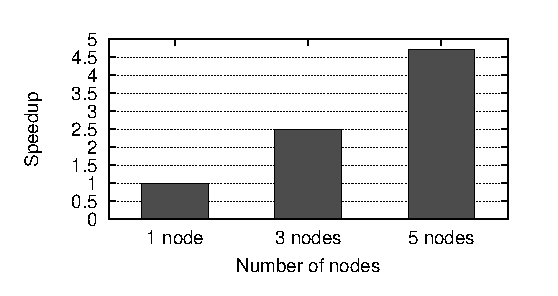
\includegraphics[width=0.35\textwidth]{chapters/mgi/grafici/graficoSpeedup.eps}
\caption{Speedup on the BigNetData dataset.}
\label{fig:speedup}
\end{figure}


\section{Conclusions and future perspectives}
\label{conclusion}
This paper presents a cloud-based service for discovering Misleading Generalized Itemsets from Big Data equipped with taxonomies.
To cope with Big Data the architecture has been designed to run on a distributed Hadoop architecture~\cite{Dean2008}.
A preliminary analysis of the applicability and usefulness of the proposed architecture was conducted on real Big Data 
acquired in a smart city environment and related to traffic law infractions.
However, the offered service could find application in many other application contexts, such as (i) social network analysis, 
(ii) network data analysis, and (iii) financial data analysis. 
As future work, we aim at optimizing and extending the current Hadoop architecture as well as testing its applicability in other real-life contexts. 
